%=======================================================================
\Tut\chapter{Mengen, Alphabete, Abbildungen}
\label{k:alphabete}

\begin{tutorium}
  \paragraph{Allgemeiner wichtiger Hinweis}

  Ab diesem Jahr ist die Vorlesung dreistündig. Wir machen
  insbesondere viel ausführlicher Aussagenlogik und Prädikatenlogik.
  (Kapitel 5 und 6)

  \emph{Bis dahin benutzen wir NICHT die Zeichen $\land$ und $\lor$
    und so weiter, sondern schreiben das IMMER ALLE schön aus und wir
    benutzen auch noch NICHT die Quantoren $\forall$ und $\exists$.}
\end{tutorium}
\begin{window}[0,r,\includegraphics[width=30mm]{../k-03-alphabete/champollion_2},{}]
\noindent Im \hyperref[k:signale]{Kapitel über Signale, Nachrichten, \dots\ \usw}
haben wir auch über \emph{Inschriften} gesprochen.
%
Ein typisches Beispiel ist der Rosetta-Stein (Abb.~\ref{abb:rosetta}),
der für \personname{Jean-François
  Champollion}%\marginpar{\includegraphics[width=20mm]{../k-03-alphabete/champollion_2}}%
\index{Champollion, Jean-Francois} \emph{die} Hilfe war, um die
Bedeutung ägyptischer Hieroglyphen zu entschlüsseln.
%
Auf dem Stein findet man Texte in drei Schriften: in Hieroglyphen, in
demotischer Schrift und auf Altgriechisch in griechischen
Großbuchstaben.
\end{window}

\begin{figure}[h]
  \centering
  \includegraphics[scale=0.8]{../k-03-alphabete/rosetta}
  \caption{Der Rosetta-Stein, heute im Britischen Museum,
    London. Bildquelle:
    \url{http://www.gutenberg.org/ebooks/48649} (17.9.15)}
  \label{abb:rosetta}
\end{figure}

Wir sind gewohnt, lange Inschriften aus (Kopien der) immer wieder
gleichen Zeichen zusammenzusetzen.
%
Zum Beispiel in europäischen Schriften sind das die Buchstaben, aus
denen Wörter aufgebaut sind.
%
Im asiatischen Raum gibt es Schriften mit mehreren Tausend Zeichen,
von denen viele jeweils für etwas stehen, was wir als Wort bezeichnen
würden.

Einen Vorrat an Zeichen, aus denen Texte zusammengesetzt werden, nennt
man ein Alphabet.
%
Das ist etwas präziser gesagt eine endliche Menge von Zeichen.

Daher werden wir in diesem Kapitel zuerst einige Anmerkungen zum
Begriff der \emph{Menge} machen.
%
Anschließend werden wir insbesondere auf zwei wichtige Alphabete der
Informatik zu sprechen kommen.
%
Das wird dann auch gleich motivieren, warum wir uns mit
\emph{Relationen} und \emph{Abbildungen} beschäftigen.

% -----------------------------------------------------------------------
\Tut\section{Mengen}
\label{subsec:mengen}

Jede Menge kann man sich als einen "`Behälter"' vorstellen, der
"`Objekte"' enthält, zum Beispiel die Menge, die die Zahlen $1$,
$2$ und $3$ enthält und nichts sonst.
%
Man sagt dann, dass $1$ ein Element dieser Menge ist, und ebenso
$2$ und $3$,
aber keine anderen Objekte.
%
Weder ist die $42$ oder eine andere Zahl ein Element der Menge, noch andere
"`andersartige"' Objekte wie zum Beispiel der linke Schuh des Autors
dieser Zeilen zu der Zeit, als er diese Zeilen schrieb.\footnote{eine
  blaue Sandale}

An vielen Stellen\graffito{\textcolor{red!50!black}{eine ganz wichtige
    allgemeine Bemerkung}} in diesem Vorlesungsskript (und allgemein
in der Mathematik und Informatik) steht man vor dem Problem, dass man
über Dinge reden möchte, die nur (mehr oder weniger) mühsam (sprich:
länglich) zu beschreiben sind.
%
Statt dann immer wieder die längliche Beschreibung zu wiederholen,
vergibt man eine \mdefine{Namen} dafür.
%
Zum Beispiel hätten wir oben sagen können:
%
\begin{quote}
  \emph{"`\ldots\ zum Beispiel die Menge $A$, die die Zahlen $1$,
    $2$ und $3$ \dots \\
    Man sagt dann, dass $1$ ein Element von $A$ ist \dots"'}
\end{quote}
%
Damit ist $A$ schlicht eine Abkürzung für etwas Längeres.
%
Es ist ein Name für etwas ganz bestimmtes.

In einem zweiten Schritt geht man bei der Benutzung von Namen noch weiter.
%
Gehen wir davon aus, dass $A$ der Name für obige Menge ist.
%
Dann sagt man auch so etwas wie: \emph{"`Es sei $x$
  ein Objekt, das in $A$ enthalten ist."'}
%
Hier wird ein neuer Name eingeführt, nämlich "`$x$"'.
%
Damit wird jetzt aber \emph{kein} ganz bestimmtes Objekt bezeichnet,
das in $A$ enthalten ist.
%
Vielmehr ist so etwas gemeint wie:
%
\begin{quote}
  \emph{"`Wir nehmen jetzt ein beliebiges Objekt her, das in $A$
    enthalten ist. Es ist gleichgültig, welches es ist. Wir nennen es
    $x$."'}
\end{quote}
%
Wenn dann im weiteren Verlauf in einer Aussage von "`$x$"'
die Rede ist, ist das eine Art Platzhalter, und man sollte sich klar
machen, dass man ihn durch jedes konkrete Objekt ersetzen kann, das in
$A$ enthalten ist.

Es sei $A$ eine Menge und $x$ ein Objekt.
%
Dann heißt $x$ \mdefine[Element einer Menge]{Element} von $A$,
wenn es in $A$ enthalten ist, und sonst nicht.
%
Wir bezeichnen mit
\[ x \in A \]
die Aussage, die wahr ist, wenn $x$
Element von $A$
ist, und andernfalls falsch.
%
Mit \[ x \notin A \] bezeichnen wir das Gegenteil von $x \in A$, also die Aussage, die genau dann wahr ist, wenn $x$ nicht Element von $A$ ist.
%
% Das wird dann üblicherweise in der Form
% \[
%   x \in A
% \]
% notiert und das Gegenteil in der Form
% \[
%   x \notin A \;.
% \]
%
Je nachdem, für welche konkreten Werte die Namen $x$
und $A$
stehen, ist also immer eine der beiden Aussagen wahr und die andere
falsch.

Anstelle von “Es sei $x$ ein Element von $A$” (und “Es sei $x$ ein Objekt so, dass $x \in A$ wahr ist") schreiben wir abkürzend “Es sei $x \in A$”.

Jede Menge soll durch die Elemente, die sie enthält, eindeutig
bestimmt sein:
%
Für zwei Mengen $A$ und $B$ ist also genau dann $A=B$, wenn für jedes Objekt $x$
gilt:
\[
  \text{ wenn } x\in A \text{, dann } x\in B \text{\quad und\quad wenn }
  x\in B \text{, dann } x\in A \;.
\]
%
Ist jedes Element einer Menge $A$ auch Element einer Menge $B$, dann
schreiben wir $A\subseteq B$ und sprechen davon, dass \mdefine[Teilmenge]{$A$
  Teilmenge von $B$} sei und $B$ \mdefine{Obermenge} von $A$.
%
Folglich gilt
\begin{lemma}
  \label{lem:mengen-gleichheit}
  Für beliebige Mengen $A$ und $B$ ist
  \[
    \text{genau dann } A=B \text{, wenn } A\subseteq B \text{ und } B\subseteq A \;.
  \]
\end{lemma}

\noindent
Kleine endliche Mengen kann man angeben, indem man alle Elemente
aufzählt.
%
Wir schließen die Aufzählung aller Elemente einer Menge in
geschweifte Klammern ein:
\[
  \{ 1, 2, 3, 4, 5, 42, \literal{A}, \literal{B} \} \;.
\]
%
Die kleinste Menge enthält gar keine Elemente.
%
Für sie schreibt man
\[
  \{\; \} \text{\qquad oder\qquad} \emptyset
\]
%
und spricht von der \mdefine[leere Menge]{leeren Menge}.

% Da die Elemente einer Menge nicht geordnet sind, macht es keinen
% Unterschied, in welcher Reihenfolge man die Elemente hinschreibt:
% \[
%   \{ 1,2,3 \} = \{ 3,2,1 \}
% \]
%
Man beachte, dass man die gleiche Menge verschieden hinschreiben kann:
\[
  \{ 1,2,3 \} = \{ 3,2,1 \} = \{ 1,1,2,3,3,2,1,3,3,3 \} \;.
\]
%
Unsere Definition der Gleichheit von Mengen verlangt nur, dass sie
jeweils die gleichen Elemente enthalten müssen.

Bei großen oder gar unendlichen Mengen kann man nicht explizit alle
Elemente einzeln auf"|führen.
%
In solchen Fällen gehen wir anders vor.
%
Zum einen setzen wir manche unendlichen Mengen einfach als bekannt voraus.
%
Für die Menge der positiven ganzen Zahlen schreiben wir $\N_+$ und für
die Menge der nichtnegativen ganzen Zahlen $\N_0$.
%
Es ist also sozusagen
\[
  \N_+ = \{ 1, 2, 3, 4, \dots \} \text{ und }
  \N_0 = \{ 0, 1, 2, 3, 4, \dots \} \;,
\]
wenn man einmal unterstellt, dass die Pünktchen von allen Lesern
"`richtig"' interpretiert werden.

Eine Möglichkeit auch unendliche Menge präzise zu spezifizieren bietet
eine Notation, die im Englischen \mdefine{set comprehension} heißt und
für wir keine gute deutsche Bezeichnung
kennen.%
\footnote{Die deutsche Bezeichnung "`Intensionale Mengennotation"' ist nicht weit verbreitet.}
%
Dafür benötigt man für jedes Element $x$ einer gewissen Grundmenge
$M$ eine Aussage $P(x)$, die wahr oder falsch ist.
%
(Wenn $P(x)$ wahr ist, sagen wir auch, "`$P(x)$ gilt"'.)
%
Dann bezeichnet $\{ x\in M \mid P(x) \}$ die Menge derjenigen Elemente
$x\in M$, für die die Aussage $P(x)$ wahr ist, \dh für jedes $y\in M$
gilt:
\[
  y \in \{ x \in M \mid P(x) \} \text{ genau dann, wenn } P(y) \text{ wahr ist} \;.
\]
%
Man liest das zum Beispiel als \emph{"`die Menge aller $x \in M$, für die
  $P(x)$ wahr ist"'}.
%
Zum Beispiel ist
\[
  \{ x \in \N_+ \mid \text{$x$ ist ohne Rest durch $2$ teilbar} \}
\]
die Menge aller positiven geraden Zahlen.
%
Wenn die Grundmenge $M$ aus dem Kontext eindeutig hervorgeht, schreiben wir abkürzend
$\{x\mid P(x)\}$.

Für zwei Mengen $A$ und $B$ ist die \mdefine{Vereinigung} $A\cup B$
eine Menge, die durch die Forderung eindeutig bestimmt ist, dass für
jedes Objekt $x$ gilt:
\[
  x\in A \cup B \text{ genau dann, wenn } x\in A \text{ oder } x \in B \;.
\]
Dabei meinen wir mit "`oder"' das inklusive Oder:
%
Es ist auch erlaubt, dass $x$ Element beider Mengen ist.
%
Der \mdefine{Durchschnitt} $A\cap B$
ist eine Menge, die durch die Forderung eindeutig bestimmt ist, dass für jedes Objekt $x$ gilt:
\[
  x\in A \cap B \text{ genau dann, wenn } x\in A \text{ und } x \in B \;.
\]
%
Es sei noch einmal daran erinnert, dass sozusagen jedes Element einer
Menge immer nur "`\emph{einmal} enthalten"' ist.
%
Daher ist zum Beispiel
\[
  \{ 1,2,3\} \cup \{3,4,5\} = \{1,2,3,4,5\} \;.
\]
%
\begin{tutorium}
  \paragraph{Vereinigung und Durchschnitt (1)}

  \begin{itemize}
  \item Deutlich darauf hinweisen: $\{ 1,2,3\} \cup \{2,3,4\}= \{1,2,3,4\}$
  \item kein Element kann "`mehrfach vorkommen"'
  \item so etwas wie $\{1,2,3,2,3,4\}$
    \begin{itemize}
    \item darf man schreiben
    \item aber es bedeutet einfach $\{1,2,3,4\}$
    \item wer so schreibt muss sich fragen, ob er schon alles
      verstanden hat
    \end{itemize}
  \item $M \cup \{\} = M$
  \item $M \cap \{\} = \{\}$
  \end{itemize}
\end{tutorium}
%
Zwei Mengen, deren Durchschnitt die leere Menge ist, nennt man \mdefine[disjunkte
Mengen]{disjunkt}.

Allgemein ist zum Beispiel für jede Menge $A$ stets $A\cup A=A$.
%
Diese und weitere Aussagen sind in den folgenden Lemmata
zusammengefasst.
%
\begin{lemma}
  \label{lem:mengen-idempotenz}
  Für jede Menge $A$ ist $A\cup A=A$ und $A\cap A=A$.
\end{lemma}

\begin{lemma}
  \label{lem:mengen-kommutativitaet}
  Für alle Mengen $A$ und $B$ ist $A\cup B=B\cup A$ und
  $A\cap B = B\cap A$.
\end{lemma}

\begin{lemma}
  \label{lem:mengen-meet-join}
  Für alle Mengen $A$ und $B$ ist $A\subseteq A\cup B$ und
  $A\cap B \subseteq A$.
\end{lemma}

\begin{lemma}
  \label{lem:mengen-assoziativitaet}
  \raggedright
  Für alle Mengen $A$, $B$ und $C$ ist
  $(A\cup B) \cup C=A\cup(B\cup C)$ und
  $(A\cap B) \cap C=A\cap(B\cap C)$.
\end{lemma}
%
Einer der wichtigsten Aspekte der Vorlesung "`Grundbegriffe der
Informatik"' ist, dass Sie lernen, präzise zu formulieren und zu
argumentieren.
%
Denn ein Algorithmus muss nicht nur präzise aufgeschrieben werden.
%
Man muss auch nachweisen können, dass es das tut, "`was er soll"'.
%
Dafür muss übrigens auch die Spezifikation präzise aufgeschrieben
sein.
%
Unter anderem aus diesem Grund werden wir in dieser Vorlesung viele
Aussagen beweisen.

Die obigen Lemmata sind aber alle recht einfach.
%
Deswegen beschränken wir uns hier auf einen Fall:
%
\begin{beweis}[erster Teil von Lemma~\ref{lem:mengen-idempotenz}]
  Es sei $A$ eine Menge. Um zu beweisen, dass $A=A\cup A$ ist,
  müssen wir nach Lemma~\ref{lem:mengen-gleichheit} zeigen:
  %
  \begin{enumerate}
  \item $A\subseteq A\cup A$
  \item $A\cup A\subseteq A$
  \end{enumerate}
  %
  Sehen wir uns die beiden Fälle nacheinander an:
%
  \begin{enumerate}
  \item Wir müssen zeigen: Jedes Element $x\in A$ ist auch Element von
    $A\cup A$.
    %
    Wenn man das ausführlich aufschreibt, ergibt sich in etwa
    folgendes:
    \begin{itemize}
    \item \emph{Es sei $x\in A$.} \\
      Wir beginnen mit der Voraussetzung.
      %
      Und um zu zeigen, dass die Aussage für jedes Element gilt,
      argumentieren wir für ein "`beliebiges"' Element, für das keine
      weiteren Annahmen gemacht werden.
    \item \emph{Dann ist $x\in A$ oder $x\in A$.}\\
      Wir ziehen eine einfache Schlussfolgerung, der unser
      umgangssprachliches Verständnis von "`oder"' zugrunde liegt.
    \item \emph{Also ist $x\in A\cup A$.} \\
      Diese Schlussfolgerung ist gerade das, was per Definition von
      Mengenvereinigung gelten muss, damit die Behauptung stimmt.
    \end{itemize}
  \item Die umgekehrte Richtung ist genauso einfach:
    %
    Wir müssen zeigen: Jedes Element $x\in A\cup A$ ist auch Element
    von $A$.
    %
    Die Struktur der Argumentation ist ähnlich wie eben:
    \begin{itemize}
    \item \emph{Es sei $x\in A\cup A$.} \\
      Wir beginnen wieder mit einem "`beliebigen"' Element.
    \item \emph{Dann ist $x\in A$ oder $x\in A$.} \\
      Das ergibt sich aufgrund der Definition von Mengenvereinigung.
    \item \emph{Also ist $x\in A$.} \\
    \end{itemize}
  \end{enumerate}
\end{beweis}
%
\begin{tutorium}
  \paragraph{Vereinigung und Durchschnitt (2)}

  Man mache sich klar: $A\cup(B \cup C)=(A\cup B)\cup C$
  (analog für Durchschnitt)

  Man mache sich klar: $A\cup(B \cap C)=(A\cup B)\cap (A\cap C)$
  (analog für Vertauschung von $\cup$ und $\cap$)
\end{tutorium}
%
Neben Vereinigung und Durchschnitt ist gelegentlich auch noch die
\mdefine{Mengendifferenz} $A\smallsetminus B$ nützlich:
\begin{align*}
  A \smallsetminus B &= \{ x\in A \mid x \notin B \} \;.
\end{align*}
%
Es ist zum Beispiel
\[
  \{ 1,2,3\} \smallsetminus \{3,4,5\} = \{1,2\} \;.
\]
%
In der nachfolgenden Abbildung~\ref{fig:zwei-mengen} sind für zwei
"`allgemeine"' Mengen $A$ und $B$ die Lage einiger Teilmengen
dargestellt.
%
Es fehlt $A\cup B$; machen Sie sich klar, welcher Bereich des Bildes
dazu gehört.
%
\begin{figure}[ht]
  \centering
  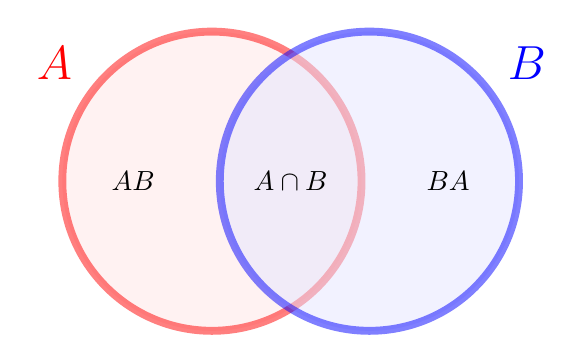
\begin{tikzpicture}
    \tikzset{venn circle/.style={draw=#1,line width=1mm,circle,minimum width=38mm,fill=#1!10!white,opacity=0.5}}

    \node [venn circle = red] (A) at (0,0) {};
    \node [venn circle = blue] (B) at (2,0) {};
    \node at (-1,0) {$A \smallsetminus B$};
    \node at (3,0) {$B \smallsetminus A$};
    \node at (barycentric cs:A=1/2,B=1/2 ) {$A \cap B$};

    \node (AA) at (-2,1.5) {\LARGE\color{red}$A$};
    \node (BB) at (4,1.5) {\LARGE\color{blue}$B$};
  \end{tikzpicture}
  %
  \caption{Teile zweier Mengen. Die linke, rote Kreisscheibe stelle
    eine Menge $A$ dar und die rechte, blaue Kreisscheibe eine Menge
    $B$.}
  \label{fig:zwei-mengen}
\end{figure}
%
\begin{tutorium}
  \paragraph{Mengendifferenz}

  Es seien $A$ und $B$ beliebige Mengen.
  %
  Man mache sich klar, dass dann die beiden folgenden Aussagen
  äquivalent sind:
  \begin{itemize}
  \item $A\smallsetminus B =\{\}$
  \item $A\subseteq B$
  \end{itemize}
\end{tutorium}


Die Anzahl der Elemente einer Menge $A$ bezeichnet man auch als ihre
\mdefine{Kardinalität}, für die wir meist
\[
  |A| \text{\qquad (oder vereinzelt  $\mathop{\mathrm{card}} A$ )}
\]
schreiben werden.
%
Für jede endliche Menge $A$ ist das offensichtlich eine nichtnegative
ganze Zahl.
%
Für unendliche Mengen werden wir nicht definieren, was $|A|$ ist, und
vermeiden darüber zu reden.

\begin{tutorium}
  \paragraph{Kardinalität}

  \begin{itemize}
  \item für endliche Mengen ist das Konzept harmlos
    \begin{itemize}
    \item vielleicht mit Ausnahme der leeren Menge: $|\{\}|=0$.
    \end{itemize}
  \item
    \begin{itemize}
    \item Frage: Wie groß ist $|\{1,2,3,2,3,4\}|$?
    \item Antwort: $4$ (und \emph{nicht (!)} $6$)
    \end{itemize}
  \item Man überlege, was man allgemein über $|A\cup B|$ sagen kann
    (vergleiche Abbildung~3.2 im Skript):
    \[
      |A\cup B| = |A| + |B| - |A\cap B|
    \]
  \end{itemize}
\end{tutorium}

%-----------------------------------------------------------------------
\Tut\section{Alphabete}
\label{subsec:alphabete}

Unter einem \mdefine{Alphabet}\index{Alphabet} wollen wir eine
endliche nichtleere Menge verstehen, deren Elemente wir \emph{Zeichen}
oder \emph{Symbole} nennen.
%
Was dabei genau "`Zeichen"' sind, wollen wir nicht weiter
hinterfragen.
%
Es seien einfach die elementaren Bausteine, aus denen Inschriften
zusammengesetzt sind.
%
Stellen Sie sich zum Beispiel einige Buchstaben des deutschen
Alphabetes vor.
%
Hier sind einfache Beispiele:
%
\begin{itemize}
\item $A=\{ \literal{|} \}$
\item $A=\{ \literal{a}, \literal{b}, \literal{c} \}$
\item $A=\{ \literal{0}, \literal{1} \}$
\item Manchmal erfindet man auch Zeichen: $A=\{ \literal{1},
  \literal{0}, \literal{\meins}\}$
\item $A=\{ \literal{0}, \literal{1}, \literal{2}, \literal{3},
  \literal{4}, \literal{5}, \literal{6}, \literal{7}, \literal{8} ,
  \literal{9}, \literal{A}, \literal{B}, \literal{C}, \literal{D},
  \literal{E}, \literal{F} \}$
\end{itemize}
%
Gelegentlich nimmt man aber auch einen etwas abstrakteren Standpunkt
ein und sieht zum Beispiel jeden der folgenden "`Kästen"' als jeweils
\emph{ein} Zeichen eines gewissen Alphabetes an:

\kasten{int} \kasten{adams} \kasten{=} \kasten{42} \kasten{;} \\
%
So etwas wird Ihnen zum Beispiel in Vorlesungen über Übersetzerbau
wieder begegnen.

Bereits in dieser Vorlesung werden wir im
\hyperref[k:aussagenlogik]{Kapitel über aussagenlogische Formeln}
annehmen, dass das zugrunde liegende Alphabet Symbole
$\mathtt{P}_{\mathtt1}$, $\mathtt{P}_{\mathtt2}$, $\mathtt{P}_{\mathtt3}$, \usw enthält.
%
Oder Sie stellen sich vor, man hätte nur die Symbole $\texttt{P}$
sowie die zehn Indexziffern ${}_{\mathtt0}$, ${}_{\mathtt1}$, ${}_{\mathtt2}$, \ldots,
${}_{\mathtt9}$, aus denen die "`eigentlichen"' grundlegenden syntaktischen
Bausteine zusammengesetzt sind.


\begin{tutorium}
  Ein Alphabet ist eine \emph{endliche}, \emph{nichtleere} Menge von
  \emph{Zeichen}.

  Was ein Zeichen ist, wird nicht weiter diskutiert, hinterfragt,
  o.ä., weshalb man letzten Endes "`theoretisch"' \emph{jede} endliche
  nichtleere Menge als Alphabet nehmen könnte.
\end{tutorium}


%-----------------------------------------------------------------------
\subsection{Beispiel ASCII}
\label{subsec:ascii}

Ein wichtiges Alphabet ist der sogenannte
\mdefine{ASCII}-Zeichensatz\index{ASCII}. Die Abkürzung steht für \emph{American
  Standard Code for Information Interchange}. Diese Spezifikation
umfasst insbesondere eine Liste von 94 "`druckbaren"' und einem
"`unsichtbaren"' Zeichen, die man \zB in Emails verwenden
darf. Außerdem hat jedes Zeichen eine Nummer aus dem Bereich der
natürlichen Zahlen zwischen $32$ und $126$. Die vollständige Liste
findet man in Tabelle~\ref{tab:ascii}.  Wie man dort sieht, fehlen in
diesem Alphabet etliche Buchstaben aus nichtenglischen Alphabeten, wie
zum Beispiel \literal{ä}, \literal{\c{c}}, \literal{\`e},
\literal{\u{g}}, \literal{\~{n}}, \literal{\oe}, \literal{ß},
\literal{\r{u}} \usw, von Kyrillisch, Japanisch und vielen anderen
außereuropäischen Schriften ganz zu schweigen.

\begin{table}[htb]
  \centering
  \begin{tabular}[t]{*{10}{c}} % *{5}{>{$}r<{$}}c@{\hspace*{3em}}}
    \toprule
       &            & 40 & \ascii{40} & 50 & \ascii{50} & 60 & \ascii{60} & 70 & \ascii{70}\\
       &            & 41 & \ascii{41} & 51 & \ascii{51} & 61 & \ascii{61} & 71 & \ascii{71}\\
    32 & \ascii{32} & 42 & \ascii{42} & 52 & \ascii{52} & 62 & \ascii{62} & 72 & \ascii{72}\\
    33 & \ascii{33} & 43 & \ascii{43} & 53 & \ascii{53} & 63 & \ascii{63} & 73 & \ascii{73}\\
    34 & \ascii{34} & 44 & \ascii{44} & 54 & \ascii{54} & 64 & \ascii{64} & 74 & \ascii{74}\\
    35 & \ascii{35} & 45 & \ascii{45} & 55 & \ascii{55} & 65 & \ascii{65} & 75 & \ascii{75}\\
    36 & \ascii{36} & 46 & \ascii{46} & 56 & \ascii{56} & 66 & \ascii{66} & 76 & \ascii{76}\\
    37 & \ascii{37} & 47 & \ascii{47} & 57 & \ascii{57} & 67 & \ascii{67} & 77 & \ascii{77}\\
    38 & \ascii{38} & 48 & \ascii{48} & 58 & \ascii{58} & 68 & \ascii{68} & 78 & \ascii{78}\\
    39 & \ascii{39} & 49 & \ascii{49} & 59 & \ascii{59} & 69 & \ascii{69} & 79 & \ascii{79}\\
    \midrule
    80 & \ascii{80} & 90 & \ascii{90} & 100 & \ascii{100} & 110 & \ascii{110} & 120 & \ascii{120} \\
    81 & \ascii{81} & 91 & \ascii{91} & 101 & \ascii{101} & 111 & \ascii{111} & 121 & \ascii{121} \\
    82 & \ascii{82} & 92 & \ascii{92} & 102 & \ascii{102} & 112 & \ascii{112} & 122 & \ascii{122} \\
    83 & \ascii{83} & 93 & \ascii{93} & 103 & \ascii{103} & 113 & \ascii{113} & 123 & \ascii{123} \\
    84 & \ascii{84} & 94 & \ascii{94} & 104 & \ascii{104} & 114 & \ascii{114} & 124 & \ascii{124} \\
    85 & \ascii{85} & 95 & \ascii{95} & 105 & \ascii{105} & 115 & \ascii{115} & 125 & \ascii{125} \\
    86 & \ascii{86} & 96 & \ascii{96} & 106 & \ascii{106} & 116 & \ascii{116} & 126 & \ascii{126} \\
    87 & \ascii{87} & 97 & \ascii{97} & 107 & \ascii{107} & 117 & \ascii{117} \\
    88 & \ascii{88} & 98 & \ascii{98} & 108 & \ascii{108} & 118 & \ascii{118} \\
    89 & \ascii{89} & 99 & \ascii{99} & 109 & \ascii{109} & 119 & \ascii{119} \\
    \bottomrule
  \end{tabular}
  \caption{Die "`druckbaren"' Zeichen des ASCII-Zeichensatzes
    (einschließlich Leerzeichen)\index{ASCII!Tabelle}}
  \label{tab:ascii}
\end{table}

%
Auf ein Zeichen in Tabelle~\ref{tab:ascii} sei ausdrücklich
hingewiesen, nämlich das mit Nummer $32$. Das ist das
"`Leerzeichen"'. Man gibt es normalerweise auf einer Rechnertastatur
ein, indem man die extrabreite Taste ohne Beschriftung drückt. Auf dem
Bildschirm wird dafür in der Regel \emph{nichts} dargestellt. Damit
man es trotzdem sieht und um darauf aufmerksam zu machen, dass das ein
Zeichen ist, ist es in der Tabelle als \ascii{32} dargestellt.

%-----------------------------------------------------------------------
\subsection{Beispiel Unicode}

Der Unicode Standard (siehe auch \url{http://www.unicode.org})
definiert mehrere Dinge. Das wichtigste und Ausgangspunkt für alles
weitere ist eine umfassende Liste von Zeichen, die in der ein oder
anderen der vielen heute gesprochenen Sprachen (\zB in Europa, im
mittleren Osten, oder in Asien) benutzt wird. Die Seite
\url{http://www.unicode.org/charts/} vermittelt einen ersten Eindruck
von der existierenden Vielfalt.

Das ist mit anderen Worten ein Alphabet, und zwar ein großes: es
umfasst rund 100\,000 Zeichen.

%Jedes Zeichen hat einen Namen. \ZB beschreibt "`\textsc{latin small
%  letter c with cedilla}"' das Zeichen \literal{\c{c}}.

Der Unicode-Standard spezifiziert weitaus mehr als nur einen
Zeichensatz.\footnote{Hinzu kommt etwa die Sortierreihenfolge von Buchstaben in verschiedenen Sprachen.
  % (im Schwedischen kommt zum Beispiel \literal{ö} \emph{nach} \literal{z}, im
  % Deutschen kommt \literal{ö} \emph{vor} \literal{z}), Zuordnung von Groß- zu
  % Kleinbuchstaben und umgekehrt (soweit existent), und vieles mehr.
}
%
Für uns sind hier zunächst nur die beiden folgenden Aspekte wichtig:

\begin{enumerate}
\item \label{pkt:unicode-alphabet} Es wird eine große (aber endliche)
  Menge $A_U$ von Zeichen festgelegt, und
\item \label{pkt:unicode-liste} eine Nummerierung dieser Zeichen,
  jedenfalls in einem gewissen Sinne.
\end{enumerate}
%
Punkt~\ref{pkt:unicode-alphabet} ist klar.
%
Hinter der Formulierung von Punkt~\ref{pkt:unicode-liste} verbirgt
sich genauer folgendes: Jedem Zeichen aus $A_U$ ist eine nichtnegative
ganze Zahl zugeordnet, der auch sogenannte \emph{Code Point} des
Zeichens. Die Liste der benutzten Code Points ist allerdings nicht
"`zusammenhängend"'.

Jedenfalls liegt eine Beziehung zwischen Unicode-Zeichen und
nichtnegativen ganzen Zahlen vor. Man spricht von einer Relation.
(Wenn Ihnen die folgenden Zeilen schon etwas sagen: schön. Wenn nicht,
gedulden Sie sich bis Abschnitt~\ref{subsec:rel-func} wenige Zeilen
weiter.)

Genauer liegt sogar eine Abbildung $f:A_U -> \N_0$ vor.  Sie ist
\begin{itemize}
\item eine Abbildung, weil jedem Zeichen nur \emph{eine} Nummer
  zugewiesen wird,
\item injektiv, weil verschiedenen Zeichen verschiedene Nummern
  zugewiesen werden,
\item aber natürlich nicht surjektiv (weil $A_U$ nur endlich viele
  Zeichen enthält).
\end{itemize}
%
Entsprechendes gilt natürlich auch für den ASCII-Zeichensatz.

%-----------------------------------------------------------------------
\Tut\section{Relationen und Abbildungen}
\label{subsec:rel-func}

%-----------------------------------------------------------------------
\Tut\subsection{Paare, Tupel und kartesische Produkte}

Es seien $A$ und $B$ zwei Mengen. Für Elemente $a\in A$ und $b\in B$ wird durch
\[
  (a,b)
\]
etwas notiert, was man als \mdefine{Paar}\index{Paar}, \emph{geordnetes Paar}\index{geordnetes Paar} oder \mdefine{Tupel}\index{Tupel} bezeichnet.
%
Der Teil $a$ vor dem Komma heißt \emph{erste Komponente} des Paares und der Teil $b$ nach dem Komma \emph{zweite Komponente}.

Zwei Paare $(a,b)$ und $(x,y)$ sind genau dann gleich, wenn $a=x$ ist
und $b=y$.
%
Also sind $(1,2)$ und $(2,1)$ \emph{verschiedene} Paare.
%
Außerdem können erste und zweite Komponente eines Paares durchaus
gleich sein.
%
Auch $(1,1)$ ist ein Paar mit zwei Komponenten.
%
\begin{tutorium}
  \paragraph{Paare}

  Bitte noch mal Unterschiede zwischen Paaren und Menge klar machen
  \[
    (1,2) \not= (2,1) \text{ \quad aber \quad } \{1,2\} = \{2,1\}
  \]
\end{tutorium}

\begin{samepage}
Das \mdefine[kartesisches\\Produkt]{kartesische
  Produkt}\index{kartesisches Produkt}\index{Produkt!kartesisches} der
Mengen $A$
und $B$,
geschrieben $A\x B$,
ist die Menge \emph{aller} Paare $(a,b)$
mit $a\in A$ und $b\in B$: %Mit anderen Worten gilt für jedes Paar $(a,b)$:
\[
  %(a,b) \in A\x B \text{ genau dann, wenn } a\in A \text{ und } b\in B \;.
  A\x B = \{ (a,b) \mid a\in A \text{ und } b\in B \} \;.
\]
\end{samepage}
%
Hier haben Gebrauch gemacht von unserer Vereinbarung, dass man die
Grundmenge (hier aller Paare) in einer set comprehension weglassen
darf, wenn diese klar aus dem Kontext hervorgeht.
%
\begin{tutorium}
  \paragraph{Kartesisches Produkt}
  Erst mal an einfachem \emph{endlichen} Beispiel klar machen:
  \[
  \{\#a,\#b\}\x \{1,2,3\}
  = \{(\#a,1), (\#a,2), (\#a,3), (\#b,1), (\#b,2), (\#b,3) \}
  \]
\end{tutorium}
%
Manchmal ist es bequem, mit Verallgemeinerungen von Paaren zu
arbeiten, die nicht genau zwei Komponenten haben.
%
Eine Möglichkeit besteht darin, diesen allgemeineren Fall auf den
schon definierten einfachen Fall zurückzuführen:
%
Seien etwa drei Mengen $M_1$, $M_2$ und $M_3$ gegeben.
%
Dann ist $(M_1\x M_2)\x M_3$
die Menge aller Paare der Form $((x_1, x_2), x_3)$,
deren erste Komponente $(x_1, x_2)\in M_1\x M_2$
ist, und deren zweite Komponente $x_3\in M_3$ ist.
%
Um beim Schreiben Klammern zu sparen und das Ganze so lesbarer zu
machen, erlauben wir, dass man im Ausdruck $(M_1\x M_2)\x M_3$ die
Klammern weglassen darf und im Ausdruck $((x_1, x_2), x_3)$ nur die
äußeren Klammern schreiben muss.
%
Alle anderen dürfen weggelassen werden.
%
Dann ist also sozusagen
\[
  M_1\x M_2\x M_3 = \{ (x_1, x_2,x_3) \mid x_1\in M_1 \text{ und } x_2\in M_2 \text{ und } x_3\in M_3 \} \;.
\]
%
Die Elemente solcher Mengen nennt man auch \mdefine{Tripel}.
%
Wir wollen diese Vorgehensweise verallgemeinern und für jede positive ganze
Zahl $n$ so etwas wie $M_1\x M_2\x \cdots \x M_n$ definieren, aber \emph{ohne} die etwas vagen Pünktchen.
%
Dazu definieren wir erstens für jedes $n\in\N_+$ eine Menge
\[
  \P_n = \{ i \in \N_+ \mid i \leq n \} \;,
\]
und zweitens induktiv für jedes $n\in\N_+$
und alle Mengen $M_i$,
mit $i\in\P_n$,
eine Menge, die wir \emph{kartesisches Produkt von $M_i$,
  mit $i\in\P_n$}, nennen und in der Form
\[
  \bigtimes_{i\in\P_n} M_i
\]
notieren, wie folgt:
\begin{align*}
  \bigtimes_{i\in\P_1} M_i &= M_1 \;, \\
  \text{für jedes $n\in\N_+$:} \bigtimes_{i\in\P_{n+1}} M_i &= \left(\bigtimes_{i\in\P_{n}} M_i\right) \x M_{n+1} \;.
\end{align*}
%
Das ist eine sogenannte \mdefine{induktive Definition}.
%
Man definiert
%
\begin{itemize}
\item zunächst explizit, was die Notation im Fall $n=1$
  bedeuten soll, nämlich $\bigtimes_{i\in\P_1} M_i = M_1$,
  (es hat sich einfach als nützlich erwiesen, das gerade so festzulegen), und
  dann
\item wie man $\bigtimes_{i\in\P_{n+1}} M_i$
  ausrechnen kann, wenn man schon $\bigtimes_{i\in\P_{n}} M_i$ kennt.
\end{itemize}
%
Man kann nun \zB ausrechnen:
\begin{align*}
  \bigtimes_{i\in\P_2} M_i &= \left(\bigtimes_{i\in\P_{1}} M_i\right) \x M_{2} \\
  &= M_1 \x M_2 \\
  \text{dann }   \bigtimes_{i\in\P_3} M_i &= \left(\bigtimes_{i\in\P_{2}} M_i\right) \x M_{3} \\
  &= (M_1 \x M_2) \x M_3 \\
  \text{dann }   \bigtimes_{i\in\P_4} M_i &= \left(\bigtimes_{i\in\P_{3}} M_i\right) \x M_{4} \\
  &= ((M_1 \x M_2) \x M_3) \x M_4 
\end{align*}
und so weiter.
%
Es sei noch einmal daran erinnert, dass wir zur Vereinfachung die Klammern
hätten weglassen dürfen.
%
\begin{tutorium}
  \textbf{induktive Definitionen}

  \begin{itemize}
  \item muss man immer darauf achten, dass
    \begin{itemize}
    \item "`für alle Fälle"' etwas definiert wird und
    \item und nicht für den gleichen Fall widersprüchliche Dinge
      festgelegt werden (Gefahr \zB bei Fallunterscheidungen). Das nennt
      man auch \emph{Wohldefiniertheit}.
    \end{itemize}
  \item Vorläufig kommen wir erst mal mit der einfachen Vorgehensweise
    aus, dass man sich von $n$ nach $n+1$ weiterhangelt, wie bei
    \begin{align*}
      x_0     &= 0 \\
      \text{für jedes } n\in\N_0: x_{n+1} &= x_n + 2 \\
    \end{align*}
  \item Solche Definitionen kann man erst mal benutzen, um Werte
    auszurechnen. Hier also z.B.  $x_1 = 2$, $x_2 = 4$, $x_3 = 6$,
    $x_4 = 8$ \usw.  Man kommt hoffentlich auf die Hypothese:
    \[
    \text{für jedes }  n\in\N_0:  x_n = 2n
    \]
  \end{itemize}
\end{tutorium}
Man gewinnt den Eindruck, dass für jede positive ganze Zahl $n$
eindeutig festgelegt ist, was $\bigtimes_{i\in\P_{n}} M_i$ sein soll.
%
Das ist in der Tat so.
%
Machen Sie sich das in diesem Beispiel klar!

Allgemein ist es ein Faktum der Mathematik, dass eine Menge $M$, die
nur positive ganze Zahlen enthält und die Eigenschaften erfüllt,
dass
\begin{enumerate}
\item $1\in M$ ist und
\item für jedes $n\in\N_0$ gilt, dass wann immer $n\in M$ ist, dann
  auch $n+1\in M$,
\end{enumerate}
gerade die Menge $\N_+$ ist.
%
(Wenn man die postiven ganzen Zahlen axiomatisch definiert, ist das sogar gerade
eine der Forderungen.)
%
Und wenn $M$ nichtnegative ganzen Zahlen enthält und man mit $0\in\ M$ beginnen kann, dann ist $M=\N_0$.
%
Daraus ergibt sich zum einen die Möglichkeit, mit Hilfe induktiver
Definitionen überhaupt sinnvolle Festlegungen zu treffen, zum anderen
fußt darauf das Beweisprinzip der sogenannten \emph{vollständigen
  Induktion}, auf das wir in späteren Kapiteln ausführlich eingehen
und zurückgreifen werden.

Die Elemente eines kartesischen Produkts von $n$
Mengen nennt man auch \mdefine{$n$-Tupel}.\index{Tupel}
%
Falls $n$ hinreichend klein ist, schreiben wir \zB auch $M_1\x M_2\x M_3$ statt $\bigtimes_{i\in\P_3} M_i$.

Sind Mengen $M_i$, mit $i\in\P_n$ und $n\in\N_+$,
alle gleich einer Menge $M$, dann nennen wir $\bigtimes_{i\in\P_n} M_i$ \emph{$n$-faches
kartesisches Produkt der Menge $M$ mit sich selbst} und notieren dieses kurz als $M^n$.
%
Mit anderen Worten, $M^n=\bigtimes_{i\in\P_n} M$.
% Präzise gesagt sei
% \begin{align*}
%   M^1 &= M \;, \\
% \text{und für jedes $n\in\N_+$: } M^{n+1} &= M \x M^n \;.
% \end{align*}
%
\begin{tutorium}
  \paragraph{Größere kartesische Produkte}

  Beispiele machen
  \begin{itemize}
  \item $\begin{aligned}[t]
      \{0,1\}^3 &= \{ (0,0,0), (0,0,1), (0,1,0), (0,1,1) \\
      &\mathrel{\hphantom{= \{}} (1,0,0), (1,0,1), (1,1,0), (1,1,1) \}
    \end{aligned}$
  \end{itemize}
\end{tutorium}

%-----------------------------------------------------------------------
\Tut\subsection{Relationen und Abbildungen}

Die Beziehung zwischen den Unicode-Zeichen in $A_U$ und nichtnegativen
ganzen Zahlen kann man durch die Angabe aller Paare $(a,n)$, für die
$a\in A_U$ ist und $n$ der zu $a$ gehörenden Code Point, vollständig
beschreiben. Für die Menge $U$ aller dieser Paare gilt also
$U\subseteq A_U\x \N_0$.

%
Eine Teilmenge $R\subseteq A\x B$ heißt auch eine
\mdefine{Relation}\index{Relation}. Manchmal sagt man noch genauer
\mdefine[binäre Relation]{binäre}\index{binäre
  Relation}\index{Relation!binäre} Relation; und manchmal noch genauer
"`von $A$ in $B$"'.
%
Das kann man auf mehr als zwei Faktoren verallgemeinern:
%
Eine \mdefine[ternäre Relation]{ternäre}\index{ternäre
  Relation}\index{Relation!ternäre} Relation ist zum Beispiel eine
Teilmenge $R \subseteq A\x B\x C$.
%
\begin{tutorium}
\noindent
  \paragraph{Begriff der Relation}
  \begin{itemize}
  \item Des öfteren ist bei einer Relation $R\subseteq A\x B$ auch
    $A=B$; man spricht dann auch von einer Relation \emph{auf der
      Menge $A$}.
  \item Beispiel "`Kleiner-Gleich-Relation"' auf der Menge
    $M=\{1,2,3\}$, \dh als Teilmenge von $M\x M$, gegeben durch die
    Paare
    \[
    R_{\leq} = \{ (1,1), (1,2), (1,3), (2,2), (2,3), (3,3) \}
    \]
  \item Manchmal benutzt man bekanntlich lieber Infixschreibweise und
    notiert $1\leq 3$ statt $(1,3)\in R_{\leq}$.
  \item Spezialfälle $A=\emptyset$ oder/und $B=\emptyset$: dann ist
    auch $A\x B=\emptyset$ und die einzig mögliche Relation ist
    $R=\emptyset$.
  \item Beispiel für eine ternäre Relation
    $R\subseteq \N_0\x\N_0\x\N_0$
    \[
      R = \{ (x,y,z) \mid x\cdot y = z \}
    \]
  \end{itemize}
\end{tutorium}

Die durch Unicode definierte Menge $U\subseteq A_U\x \N_0$ hat
"`besondere"' Eigenschaften, die nicht jede Relation hat. Diese (und
ein paar andere) Eigenschaften wollen wir im folgenden kurz aufzählen
und allgemein definieren:

\begin{enumerate}
\item Zum Beispiel gibt es für jedes Zeichen $a\in A_U$ (mindestens)
  ein $n\in\N_0$ mit $(a,n)\in U$.

  Allgemein nennt man eine Relation $R\subseteq A\x B$
  \mdefine{linkstotal}\index{linkstotale
    Relation}\index{Relation!linkstotal}, wenn für jedes $a\in A$
  (mindestens) ein $b\in B$ existiert mit $(a,b)\in R$.
\item Für kein Zeichen $a\in A_U$ gibt es mehrere $n\in\N_0$ mit der
  Eigenschaft $(a,n)\in U$.

  Allgemein nennt man eine Relation $R\subseteq A\x B$
  \mdefine{rechtseindeutig}\index{rechtseindeutige
    Relation}\index{Relation!rechtseindeutig}, wenn es für kein $a\in
  A$ zwei $b_1\in B$ und $b_2\in B$ mit $b_1\not= b_2$ gibt so, dass
  sowohl $(a,b_1)\in R$ als auch $(a,b_2)\in R$ ist.
\item Relationen, die linkstotal und rechtseindeutig sind, kennen Sie
  auch unter anderen Namen: Man nennt sie
  \mdefine[Abbildung]{Abbildungen}\index{Abbildung} oder auch
  \mdefine[Funktion]{Funktionen}\index{Funktion} und man schreibt dann
  üblicherweise $R:A \rightarrow B$. Es heißt dann $A$ der
  \mdefine{Definitionsbereich}\index{Definitionsbereich} und $B$ der
  \mdefine{Zielbereich}\index{Zielbereich} der Abbildung.

  Gelegentlich ist es vorteilhaft, sich mit Relationen zu
  beschäftigen, von denen man nur weiß, dass sie rechtseindeutig
  sind. Sie nennt man manchmal \mdefine[partielle Abbildung]{partielle
    Abbildungen}\index{partielle
    Abbildung}\index{Abbildung!partielle}\index{Funktion!partielle}. (Bei
  ihnen verzichtet man also auf die Linkstotalität.)
\item Außerdem gibt es bei Unicode keine zwei verschiedene Zeichen
  $a_1$ und $a_2$, denen der gleiche Code Point zugeordnet ist.

  Eine Relation $R\subseteq A\x B$ heißt
  \mdefine{linkseindeutig}\index{linkseindeutige
    Relation}\index{Relation!linkseindeutig}, wenn für alle $(a_1,b_1)
  \in R$ und alle $(a_2,b_2) \in R$ gilt:
  \[
  \text{wenn } a_1\not= a_2, \text{ dann }  b_1\not=b_2 \;.
  \]
\item Eine Abbildung, die linkseindeutig ist, heißt
  \mdefine{injektiv}\index{injektive
    Abbildung}\index{Abbildung!injektiv}\index{Funktion!injektiv}.
\item Der Vollständigkeit halber definieren wir auch gleich noch, wann
  eine Relation $R\subseteq A\x B$
  \mdefine{rechtstotal}\index{rechtstotale
    Relation}\index{Relation!rechtstotal} heißt: wenn für jedes $b\in
  B$ ein $a\in A$ existiert, für das $(a,b)\in R$ ist.
\item Eine Abbildung, die rechtstotal ist, heißt
  \mdefine{surjektiv}\index{surjektive
    Abbildung}\index{Abbildung!surjektiv}\index{Funktion!surjektiv}.
\item Eine Abbildung, die sowohl injektiv als auch surjektiv ist,
  heißt \mdefine{bijektiv}\index{bijektive
    Abbildung}\index{Abbildung!bijektiv}\index{Funktion!bijektiv}.
\end{enumerate}

\begin{tutorium}
\noindent
  \paragraph{Linkstotal etc.}
  \begin{itemize}
  \item Begriffe linkstotal, rechtseindeutig und Abbildung an
    Beispielen wiederholen, Definitionen in äquivalente umformulieren,
    z.B. "`rechtstotal, wenn es kein $b\in B$ gibt, zu dem kein $a\in
    A$ in Relation steht"'
  \item Begriffe linkseindeutig/injektiv und rechtstotal/surjektiv und
    bijektiv wiederholen
  \item Begriffe Definitionsbereich, Zielbereich \\
  \item Betrachte $f:A -> A$, also Definitionsbereich gleich Zielbereich
    und A sei \emph{endlich}.
    \begin{itemize}
    \item Zeige: Wenn injektiv, dann auch surjektiv.
    \item Zeige: Wenn surjektiv, dann auch injektiv.
    \item Zeige: Wenn $A$ unendlich ist, dann stimmen diese
      Behauptungen im allgemeinen nicht mehr.

      Betrachte \zB $f:\N_0->\N_0: n \mapsto 2n$ und $g:\N_0->\N_0: n
      \mapsto \lfloor n/2\rfloor$
    \end{itemize}
  \end{itemize}
\end{tutorium}

\noindent
Im Laufe der Vorlesung wird es immer wieder notwendig sein, Abbildungen
zu definieren.
%
Dazu gehört als erstes immer die Angabe von Definitionsbereich und
Zielbereich (denn davon ist ja zum Beispiel unter Umständen abhängig,
ob eine Abbildung injektiv ist).
%
Wir notieren das wie oben erwähnt in der Form
\[
  f \colon A \to B \;.
\]
%
In dieser Situation gibt es für jedes $a\in A$
\emph{genau ein} $b\in B$ mit $(a,b)\in f$.
%
Man schreibt dann üblicherweise $f(a)=b$
und nennt $b$
den \emph{Wert} oder \mdefine{Funktionswert} von $f$
an der Stelle $a$.
%
Wenn für jedes Element $a$ des Definitionsbereichs der Funktionswert
$f(a)$ spezifiziert werden soll, schreiben wir das oft in einer der
Formen
%
\begin{align*}
  x &\mapsto \text{Ausdruck, in dem $x$ vorkommen darf,} \\
  (x,y) &\mapsto \text{Ausdruck, in dem $x$ und $y$ vorkommen dürfen,} \\
\end{align*}
%
falls der Definitionsbereich von $f$ eine Menge \bzw das kartesische
Produkt zweier Mengen ist.
%
(Wenn der Definitionsbereich kartesisches Produkt von mehr als zwei
Mengen ist, gehen wir analog vor.)
%
Im ersten Fall wird ein Name (hier $x$)
für den Wert eingeführt, auf den die Abbildung angewendet wird.
%
Im zweiten Fall wird angenommen, dass der Wert ein Paar ist, es werden sogar
Namen ($x$ und $y$)
für seine "`Bestandteile"' eingeführt und es wird darauf vertraut, dass
allen klar ist, welche Bestandteile gemeint sind.

Auf der rechten Seite der Definition von Funktionswerten erlauben wir uns die
Freiheit, nicht nur einfache arithmetische Ausdrücke zu notieren, sondern \zB
auch Fallunterscheidungen.
%
Hier ist ein einfaches Beispiel:
\[
  f \colon \N_0 \to \N_0, n \mapsto
  \begin{cases}
    n/2, & \text{ falls $n$ gerade,} \\
    3n+1, & \text{ falls $n$ ungerade.}
  \end{cases}
\]
% Alternativ schreiben wir die beiden wesentlichen Teile manchmal auch
% untereinander:
% \begin{align*}
%   f \colon \N_0 &\to \N_0, \\
%   n &\mapsto
%       \begin{cases}
%         n/2, & \text{ falls $n$ gerade,} \\
%         3n+1, & \text{ falls $n$ ungerade.}
%       \end{cases}
% \end{align*}
%
Man beachte, dass die Namen die in der Definition der Abbildung
verwendet werden, völlig irrelevant sind.
%
Genau die gleiche Abbildung wie eben wird definiert, wenn man schreibt:
\[
  g \colon \N_0 \to \N_0,  x \mapsto
  \begin{cases}
    x/2, & \text{ falls $x$ gerade,} \\
    3x+1, & \text{ falls $x$ ungerade.}
  \end{cases}
\]
%
\begin{tutorium}
  \paragraph{Notation für Abbildungen}

  Bitte bei sich selbst und bei den Tutanden darauf achten, dass
  Abbildungen immer ordentlich hingeschrieben werden:
  \begin{itemize}
  \item Definitions- und Zielbereich mit einem einfachen Pfeil $\to$
    dazwischen und
  \item Argument(e) und Funktionswert mit einem $\mapsto$ dazwischen
  \end{itemize}

  Wir werden darauf im Abschnitt zu O-Notation noch einmal
  zurückkommen.
\end{tutorium}

\noindent
Mitunter ist die folgende Verallgemeinerung der Schreibweise $f(a)$
nützlich.
%
Ist $f\colon A \to B$ und $M\subseteq A$, so sei
\[
  f(M) = \{ b \in B \mid \text{ es gibt ein } a \in M \text{ mit
  } f(a)=b \} \;.
\]
%
Das ist mühsam (zu schreiben und) zu lesen, weshalb wir folgende
verallgemeinerte Notation für \emph{set comprehensions} erlauben:
\begin{align*}
  \text{statt } &\{ b \in B \mid \text{es gibt ein $a$ mit } f(a)=b \text{ und } P(a) \} \\
  \text{kurz } &\{ f(a) \mid P(a) \} \;.
\end{align*}
%
Damit ist $f(M)=\{ f(a)\mid a\in M\}$.
%
Für eine Abbildung $f\colon A\to B$ heißt $f(A)$ auch das
\mdefine{Bild} der Abbildung.

\begin{tutorium}
  \paragraph{Notation von Abbildungen für Mengen von Argumenten}

  Beispiel für $f(M) = \{ f(a) \mid a \in M \}$ machen
\end{tutorium}

%-----------------------------------------------------------------------
\Tut\section{Mehr zu Mengen}

Elemente einer Menge können ihrerseits wieder Mengen sein.
%
Zum Beispiel enthält die Menge
\[
  M = \{\; 1, \; \{2,3\}, \; 4,\; 5,\; 6, \; \{7,8,9\}, \; \{\} \; \}
\]
\emph{sieben (!)} Elemente, von denen drei ihrerseits wieder Mengen
sind, nämlich $\{2,3\}$, $\{7,8,9\}$ und die leere Menge $\{\}$.
%
Man beachte auch, dass die Menge $\{ \;\{\}\;\}$ ein Element enthält
(die leere Menge), also selbst offensichtlich \emph{nicht} leer ist!
%
\begin{tutorium}
  \paragraph{Mengen als Elemente von Mengen}

  Unbedingt den Unterschied zwischen $\{\}$ und $\{ \;\{\}\;\}$ klar
  machen.
\end{tutorium}

Zu jeder Menge $M$ definiert man die
\mdefine[Potenz-\\menge]{Potenzmenge}\index{Potenzmenge} als die Menge \emph{aller}
Teilmengen von $M$.
%
Wir schreiben dafür $2^M$, einige andere Autoren benutzen die Notation
$\mathfrak{P}(M)$.
%
Also:
\[
  2^M = \{ A \mid A \subseteq M \} \;.
\]
%
Betrachten wir als Beispiel $M=\{1,2,3\}$.
%
Dann ist
\[
  2^{\{1,2,3\}} = \{ \{\} ,\; \{1\} ,\; \{2\} ,\; \{3\} ,\; \{1,2\}
  ,\; \{1,3\} ,\; \{2,3\} ,\; \{1,2,3\} \} \;.
\]
%
Allgemein kann man also immer statt $A\subseteq M$ auch $A\in 2^M$
schreiben; und gelgentlich tut man das auch.
%
\begin{tutorium}
  \paragraph{Potenzmenge}

  Es sei $M=\{0,1\}$.
  \begin{itemize}
  \item $2^M$ herleiten: $2^M=\{ \{\} ,\; \{0\} ,\; \{1\} ,\; \{0,1\} \;\}\} $
  \item $2^{2^M}$ herleiten:
    \begin{align*}
      2^{2^M} = \{ \; & \{\} \\
                      & \{\{\}\} ,\; \{\{0\}\} ,\; \{\{1\}\} ,\; \{\{0,1\}\} \\
                      & \{\{\},\{0\}\} ,\; \{\{\},\{1\}\} ,\; \{\{\},\{0,1\}\} ,\; \{\{0\},\{1\}\} ,\; \{\{0\},\{0,1\}\} ,\; \{\{1\},\{0,1\}\}, \\
                      & \{\{\},\{0\},\{1\}\} ,\; \{\{\},\{0\},\{0,1\}\} ,\; \{\{\},\{1\},\{0,1\}\} ,\; \{\{0\},\{1\},\{0,1\}\} ,\; \\
                      & \{\{\},\{0\},\{1\},\{0,1\}\} \\
                \} \;
    \end{align*}
  \end{itemize}
\end{tutorium}

Zu zwei beliebigen Mengen $I$ und $M$ betrachten wir nun eine Abbildung
\[
  f \colon I \to 2^M \;.
\]
%
Wenn es Ihnen die Sache erleichtert, stellen Sie sich vor, es sei \zB
$I=\P_2=\{1,2\}$ oder $I=\N_0$.
%
Es ist jedenfalls für jedes $i\in I$ der Funktionswert $f(i)$ eine
Element von $2^M$, also eine Teilmenge von $M$.
%
Statt $f(i)$ schreiben wir im Folgenden $M_i$.
%
Wenn $I=\{1,2\}$ ist, dann sind also einfach zwei Mengen $M_1$ und
$M_2$ festgelegt.
%
Und wenn $I=\N_0$ ist, dann hat man eine sogenannte \emph{abzählbar
  unendliche} Folge von Mengen (genauer Teilmengen von $M$) $M_0$,
$M_1$, $M_2$, und so weiter.

Als Verallgemeinerung von Durchschnitt und Vereinigung zweier Mengen definieren
wir die \mdefine[Vereinigung]{Vereinigung $\bigcup_{i\in I} M_i$}
und den \mdefine[Durchschnitt]{Durchschnitt $\bigcap_{i\in I} M_i$}
aller $M_i$ so:
%
\begin{align*}
  \bigcup_{i\in I} M_i &= \{ x \mid \text{es gibt ein } i\in I \text{ so, dass } x\in  M_i \}  \;,\\
  \bigcap_{i\in I} M_i &= \{ x \mid \text{für jedes } i\in I \text{ ist } x\in  M_i \} \;.\\
\end{align*}
%
Machen Sie sich bitte klar, dass im Fall $I=\{1,2\}$ gilt:
\begin{align*}
  \bigcup_{i\in I} M_i &= M_1 \cup M_2 \text{ und }\\
  \bigcap_{i\in I} M_i &= M_1 \cap M_2 \;.
\end{align*}

%-----------------------------------------------------------------------
\section*{Zusammenfassung und Ausblick}

In diesem Kapitel wurde zunächst auf den Begriff der \emph{Menge}
eingegangen und es wurden einfache Operationen mit Mengen definiert.

Dann wurde der Begriff \emph{Alphabet} eingeführt, der im weiteren
Verlauf dieser Vorlesung und des Informatikstudiums noch an vielen
Stellen eine Rolle spielen wird.
%
Wer mehr über Schriften wissen möchte, findet zum Beispiel über die
WWW-Seite \url{http://www.omniglot.com/writing/} (6.10.2015) weitere
Informationen.

Als wichtige technische Hilfsmittel wurden die Begriffe \emph{binäre
  Relation}, sowie \emph{injektive}, \emph{surjektive} und
\emph{bijektive Abbildungen} definiert.

Viele Aussagen hatten noch den Nachteil, dass sie umgangssprachlich
und daher relativ weitschweifig formuliert waren.
%
Nachdem im nächsten Kapitel die Begriffe \emph{Wort} und \emph{formale
  Sprache} eingeführt worden sein werden, werden wir uns daher
anschließend ein erstes Mal mit \emph{Aussagenlogik} und danach mit
\emph{Prädikatenlogik} (erster Stufe) beschäftigen.

\cleardoublepage

%-----------------------------------------------------------------------
%%%
%%% Local Variables:
%%% fill-column: 80
%%% mode: latex
%%% eval: (visual-line-mode 1)
%%% eval: (visual-fill-column-mode 1)
%%% TeX-master: "../k-03-alphabete/skript.tex"
%%% TeX-command-default: "XPDFLaTeX"
%%% End:
